% Created 2022-02-02 mié 21:00
% Intended LaTeX compiler: pdflatex
\documentclass[xcolor={usenames,svgnames,dvipsnames}, aspectratio=169]{beamer}
\usepackage[utf8]{inputenc}
\usepackage[T1]{fontenc}
\usepackage{graphicx}
\usepackage{grffile}
\usepackage{longtable}
\usepackage{wrapfig}
\usepackage{rotating}
\usepackage[normalem]{ulem}
\usepackage{amsmath}
\usepackage{textcomp}
\usepackage{amssymb}
\usepackage{capt-of}
\usepackage{hyperref}
\usepackage{color}
\usepackage{listings}
\usepackage[spanish]{babel}
\usecolortheme{rose}
\setbeamercolor{alerted text}{fg=DarkBlue}
\setbeamerfont{alerted text}{series=\bfseries}
\setbeamerfont{block title}{series=\bfseries}
\setbeamercolor{block title}{bg=structure.fg!20!bg!50!bg}
\setbeamercolor{block body}{use=block title,bg=block title.bg}
\setbeamertemplate{navigation symbols}{\insertsectionnavigationsymbol}
\AtBeginSection[]{\begin{frame}[plain]\tableofcontents[currentsection,sectionstyle=show/shaded]\end{frame}}
\AtBeginSubsection[]{\begin{frame}[plain]\tableofcontents[currentsubsection,sectionstyle=show/shaded,subsectionstyle=show/shaded]\end{frame}}
\lstset{keywordstyle=\color{blue}, commentstyle=\color{gray!90}, basicstyle=\ttfamily\small, columns=fullflexible, breaklines=true,linewidth=\textwidth, backgroundcolor=\color{gray!23}, basewidth={0.5em,0.4em}, literate={¡}{{\textexclamdown}}1 {á}{{\'a}}1 {ñ}{{\~n}}1 {é}{{\'e}}1 {ó}{{\'o}}1 {í}{{\'i}}1 {ú}{{\'u}}1 {º}{{\textordmasculine}}1, showstringspaces=false}
\usepackage{mathpazo}
\usepackage{siunitx}
\hypersetup{colorlinks=true, linkcolor=Blue, urlcolor=Blue}
\usepackage{fancyvrb}
\DefineVerbatimEnvironment{verbatim}{Verbatim}{fontsize=\tiny, formatcom = {\color{black!70}}}
\setbeamertemplate{footline}[frame number]
\usetheme{Boadilla}
\usefonttheme{serif}
\author{Oscar Perpiñán Lamigueiro}
\date{}
\title{Tema 1: Introducción a la Programación}
\hypersetup{
 pdfauthor={Oscar Perpiñán Lamigueiro},
 pdftitle={Tema 1: Introducción a la Programación},
 pdfkeywords={},
 pdfsubject={},
 pdfcreator={Emacs 27.1 (Org mode 9.4.6)}, 
 pdflang={Spanish}}
\begin{document}

\maketitle

\begin{frame}[label={sec:orgc01e6fa},plain]{¿Por qué programar?}
\href{https://www.youtube.com/watch?v=QvyTEx1wyOY}{\includegraphics[height=0.9\textheight]{figs/steve-jobs-quote.jpg}}
\end{frame}

\begin{frame}[label={sec:org804c2a3},plain]{¿Qué hay dentro de un ordenador?}
\href{http://www.gcflearnfree.org/computerbasics/inside-a-computer/1/}{\includegraphics[height=0.9\textheight]{figs/InsideComputer.png}}
\end{frame}

\begin{frame}[label={sec:org912da76},plain]{¿Cómo funciona un ordenador?}
\href{https://youtu.be/DKGZlaPlVLY?t=42}{\includegraphics[height=0.9\textheight]{figs/HowComputersWork.png}}
\end{frame}

\begin{frame}[label={sec:org837a026}]{Algoritmo y Programa Informático}
\begin{itemize}
\item \alert{Algoritmo}: método para resolver un problema.
\item \alert{Programa informático}:
\begin{itemize}
\item una colección de instrucciones expresadas de forma que un ordenador pueda realizar una tarea.
\item es una implementación del algoritmo para un determinado sistema informático.
\end{itemize}
\item \alert{Lenguaje máquina}: los ordenadores utilizan el sistema de numeración binario (dos dígitos, 0 y 1) para almacenar información.
\item Las instrucciones del programa deben estar codificadas como sucesiones de 0s y 1s.
\end{itemize}
\begin{center}
01001000 01101111 01101100 01100001
\end{center}
\end{frame}

\begin{frame}[label={sec:org7aefee8}]{¿Qué es un lenguaje de programación?}
Un lenguaje artificial que emplea \alert{expresiones similares al lenguaje humano} y un \alert{traductor} para convertir a código binario.
\begin{itemize}
\item Lenguaje de \alert{bajo nivel}: similar al lenguaje máquina, adaptado a un procesador concreto.
\item Lenguaje de \alert{alto nivel}: similar al lenguaje natural, de uso general.
\end{itemize}
\end{frame}

\begin{frame}[label={sec:org4868bd4},fragile]{Ejemplo de lenguaje de bajo nivel}
 \begin{block}{Ensamblador}
\begin{verbatim}
STACK	SEGMENT STACK
      	DW 64 DUP (?)
STACK 	ENDS
DATA	SEGMENT
SALUDO 	DB “Hola Mundo",13,10,"$" ; Cadena
DATA   	ENDS
CODE	SEGMENT
	ASSUME CS:CODE, DS:DATA, SS:STACK
INICIO:
	MOV AX,DATA
	MOV DS,AX
	MOV DX,OFFSET SALUDO
	MOV AH,09H
	INT 21H
	MOV AH,4CH
	INT 21H
CODE	    ENDS
	END INICIO
\end{verbatim}
\end{block}
\end{frame}

\begin{frame}[label={sec:org58ece60},fragile]{Ejemplo de lenguaje de alto nivel}
 \begin{block}{Python}
\lstset{language=Python,label= ,caption= ,captionpos=b,numbers=none}
\begin{lstlisting}
print "Hola Mundo"
\end{lstlisting}
\end{block}

\begin{block}{R}
\lstset{language=r,label= ,caption= ,captionpos=b,numbers=none}
\begin{lstlisting}
print("Hola Mundo")
\end{lstlisting}
\end{block}

\begin{block}{Más Ejemplos}
\url{https://es.wikipedia.org/wiki/Anexo:Ejemplos\_de\_implementaci\%C3\%B3n\_del\_\%C2\%ABHola\_mundo\%C2\%BB}
\end{block}
\end{frame}

\begin{frame}[label={sec:org0e901e8}]{Lenguajes de alto nivel}
\begin{center}
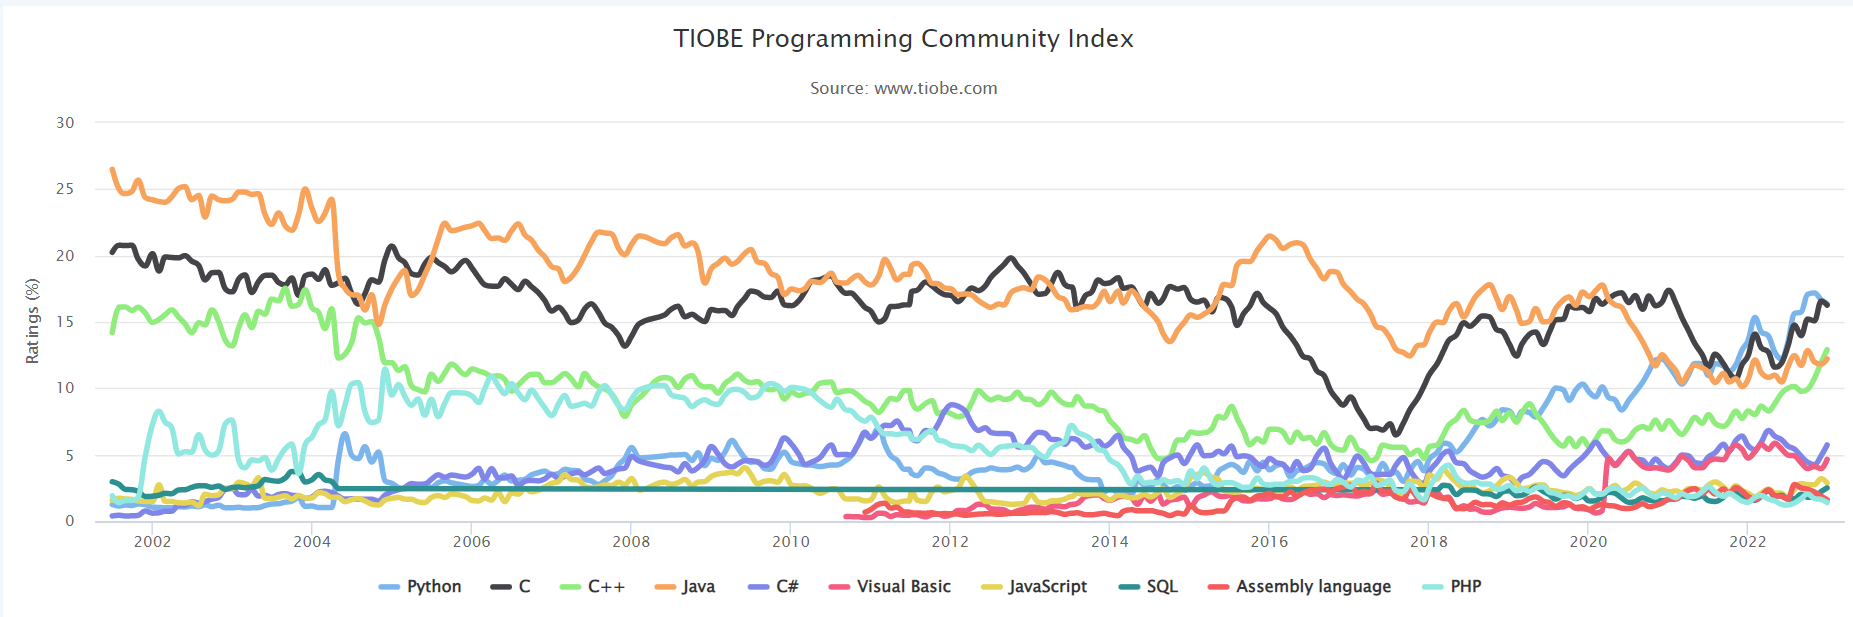
\includegraphics[width=.9\linewidth]{figs/TIOBEindex.png}
\end{center}

\url{http://www.tiobe.com/tiobe-index/}
\end{frame}

\begin{frame}[label={sec:org3aa0442}]{C}
\begin{block}{Características}
\begin{itemize}
\item Lenguaje de nivel \emph{medio}.
\item De propósito general
\item Compacto (sólo 32 palabras)
\item Estructurado. Permite reutilizar el código.
\item Funciona en plataformas diferentes.
\end{itemize}
\end{block}

\begin{block}{Historia}
\begin{itemize}
\item C (Ritchie, 1972. Laboratorios Bell).
\item ANSI C American National Standards Institute C (1989).
\item C99 (ISO/IEC 9899, 1999).
\end{itemize}
\end{block}
\end{frame}
\begin{frame}[label={sec:org1fbeea4},fragile]{Ejemplo de programa en C}
 \lstset{language=C,label= ,caption= ,captionpos=b,numbers=none}
\begin{lstlisting}
#include <stdio.h>

int main()
{
  printf("Hola Mundo\n");

  return 0;
}
\end{lstlisting}
\end{frame}
\begin{frame}[label={sec:org3f88020}]{Desarrollo de programas en C}
\begin{center}
\includegraphics[height=0.9\textheight]{figs/programaC.png}
\end{center}
\end{frame}


\begin{frame}[label={sec:org3418000}]{Cómo programar}
Extraído de \href{https://arxiv.org/pdf/1210.0530v4.pdf}{Best Practices for Scientific Computing}

\begin{itemize}
\item Write programs for people, not computers.
\item Automate repetitive tasks
\item Use the computer to record history
\item Make incremental changes
\item Use version control
\item Don't repeat yourself (or others)
\item Plan for mistakes
\item Optimize software only after it works correctly
\item Document design and purpose, not mechanics
\item Collaborate
\end{itemize}
\end{frame}
\end{document}